% !TEX root = ../main.tex
\paragraph{Forward Tagger (FT)}
    The FT is an extension of the CLAS12 detector that allows for the detection of electrons and photons at very forward polar angles, specifically ranging from $2.5\degree$ to $4.5\degree$.
    By detecting forward-scattered electrons, the FT enables electroproduction experiments at low photon virtuality $Q^2$, providing a high-intensity, linearly polarized, quasi-real photon beam with energy tagging.
    This setup is particularly suitable for hadron spectroscopy studies.

    The FT consists of three main components: the FTCal (calorimeter), the FTTrk (micro-strip gas tracker), and the FTHodo (hodoscope).
    The FTCal utilises 332 lead-tungstate ($\text{PbWO}_4$) crystals to identify electrons, measure the energy of electromagnetic showers, and provide fast trigger signals.
    The FTTrk, located in front of the FTCal, is responsible for measuring the scattering angles of charged particles.
    The FTHodo, a scintillator detector, assists in the separation of electrons and high-energy photons.

    \begin{wrapfigure}{l}{0.50\textwidth}
        \frame{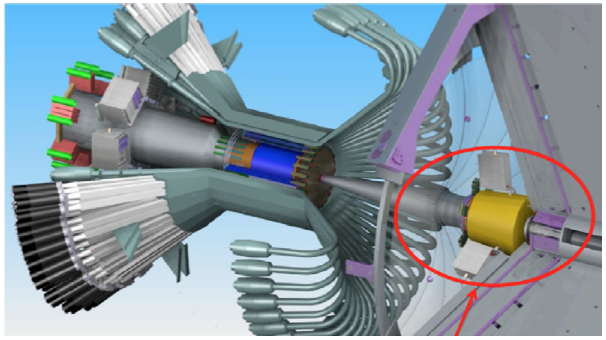
\includegraphics[width=\linewidth]{217ft.png}}
        \caption[FT]
        {The Forward Tagger (FT) system circled downstream of the CD in front of the torus magnet warm bore entrance.}
        \floatfoot{Source: \href{https://jlab.org/physics/hall-b/clas12}{CLAS12 wiki}.}
        \label{fig::11.217::ft}
    \end{wrapfigure}

    During beam operations, a conical tungsten shielding pipe is placed in front of the FT to absorb M\o ller electrons and low-energy photons generated by beam interactions with the target and downstream materials.
    This shielding not only protects the FT and Forward Detectors from electromagnetic background but also ensures compatibility with the FT acceptance.
    This configuration, referred to as ``FT-ON'', allows the FT to detect both electrons and photons, expanding the detection capabilities of CLAS12.

    Alternatively, when the FT is not required for the specific physics program, the FT detectors can be turned off, and additional shielding elements are installed in front of the FT, covering up to $4.5\degree$ of polar angle.
    This modified configuration, known as "FT-Off," reduces accidental background by one-third under the same beam conditions, enabling higher luminosity data acquisition with CLAS12 by mitigating background interference from the DC R1 chambers \cite{acker2020ft}.

    A render of the FT can be seen in Figure \ref{fig::11.217::ft}.
